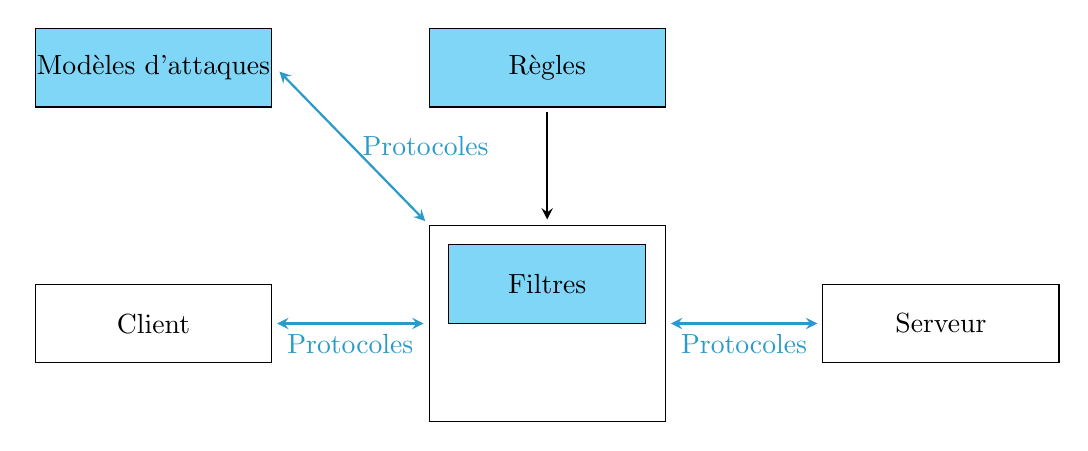
\begin{tikzpicture}[
    arrow/.style={thick,->,shorten >=2pt,shorten <=2pt,>=stealth},
    darrow/.style={thick,<->,shorten >=2pt,shorten <=2pt,>=stealth},
]

    \draw (0,.75) rectangle (3,1.75) node [pos=.5] {Client};
    
    %\fill[cyan!50!white] (5,0) rectangle (8,2.5);
    \draw (5,0) rectangle (8,2.5) node [pos=.5,below=.4] {\aramis};
    \fill[cyan!50!white] (5.25,1.25) rectangle (7.75,2.25);
    \draw (5.25,1.25) rectangle (7.75,2.25) node [pos=.5] {Filtres};
    
    \draw (10,.75) rectangle (13,1.75) node [pos=.5] {Serveur};

    \fill[cyan!50!white] (0,4) rectangle (3,5);
    \draw (0,4) rectangle (3,5) node [pos=.5] {Modèles d'attaques};

    \draw[darrow,cyan!80!black] (3.05,4.5) -- (5,2.5) node [pos=.5,right] {Protocoles};

    \fill[cyan!50!white] (5,4) rectangle (8,5);
    \draw (5,4) rectangle (8,5) node [pos=.5] {Règles};

    \draw[arrow,] (6.5,4) -- (6.5,2.5);

    \draw[darrow,cyan!80!black] (3,1.25) -- (5,1.25) node [pos=.5,below] {Protocoles};
    \draw[darrow,cyan!80!black] (8,1.25) -- (10,1.25) node [pos=.5,below] {Protocoles};

    %\draw[dashed,cyan!80!black] (-.25,-.25) rectangle (13.25,5.25);
    %\draw node [align=left,below right,cyan!80!black] at (0,5) {{\bf Attack models}};
    %\draw node [align=left,below right,cyan!80!black] at (0,4.5) {Produce attack\\scenarios given\\a system and\\attacker objectives};
\end{tikzpicture}
